\appendix
\chapter{Guida utente}
\section{Monopoly \- Guida Utente}
\subsection{Introduzione e obiettivi del gioco}
Benvenuto nel tuo Monopoly!\newline
L’obiettivo è semplice: diventare il giocatore più ricco accumulando proprietà, incassando affitti e gestendo con attenzione il proprio patrimonio.
Per farlo, i giocatori si alternano in turni scanditi dal lancio dei dadi, muovendosi sul tabellone, acquistando terreni, costruendo case e interagendo con eventi casuali.\newline
La partita può essere affrontata in due modalità:\newline
\begin{itemize}
    \item Classic Mode: richiede un'attenta gestione finanziaria e include il rischio di bancarotta.
    \item Infinity Mode: rende il gioco libero e senza eliminazioni per bancarotta.  
\end{itemize}
Il gioco supporta più giocatori, ognuno dei quali sceglie un nome e seleziona un colore tra quelli disponibili.
Il regolamento completo è sempre consultabile tramite l’apposito pulsante "?", disponibile sia nel menu iniziale che durante la partita.
\subsection{Avvio del gioco}
All’avvio, il gioco presenta un menu iniziale da cui è possibile:\newline
\begin{itemize}
    \item Avviare una nuova partita
    \item Consultare le regole
    \item Modificare il numero di giocatori
    \item Accedere alle impostazioni (Settings) per selezionare la modalità di gioco
\end{itemize}
\begin{figure}[H]
    \centering
    \makebox[0.5\textwidth]{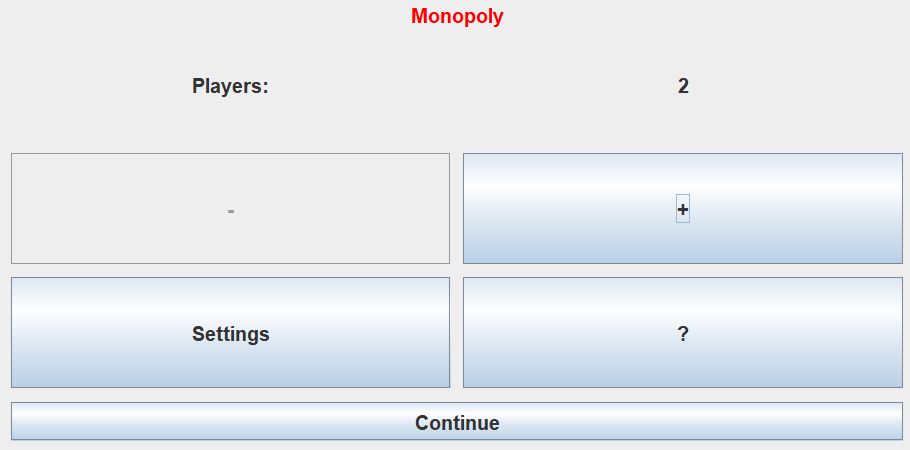
\includegraphics[width=1.3\textwidth]{img/screengame/sel_num_player.png}}	
    \caption{il menu iniziale di gioco}
	\label{img:gamescreen1}
\end{figure}
\textbf{Scelta dei giocatori}\newline
Ogni partecipante inserisce il proprio nome in corrispondenza di uno dei colori disponibili. Ogni colore rappresenta un token unico sul tabellone e identifica visivamente le proprietà acquistate.\newline
\textbf{File di configurazione\texttt{(config.yml)}:}\newline
\begin{figure}[H]
    \centering
    \makebox[0.5\textwidth]{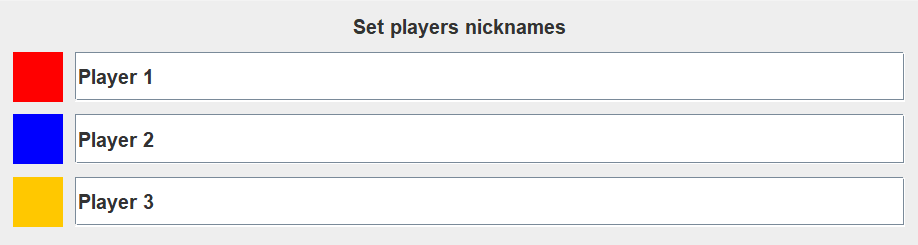
\includegraphics[width=1.3\textwidth]{img/screengame/sel_name_color_player.png}}	
    \caption{schermata di selezione nome e colore dei giocatori}
	\label{img:gamescreen2}
\end{figure}
Il gioco carica all’avvio il file \texttt{config.yml}, che definisce alcuni parametri fondamentali per la partita. Se il file non viene trovato o contiene errori di formattazione, viene caricata automaticamente una configurazione standard valida.\newline
Esempio di contenuto:\newline
\begin{verbatim}
MIN_PLAYERS: 2
MAX_PLAYERS: 6
NUM_DICE: 2
SIDES_PER_DIE: 6
FONT_NAME: SansSerif
FONT_SIZE: 20
INIT_BALANCE: 2000
RULES_FILE: rules/rules.txt
CARDS_FILE: cards/final_cards.json
DECK_FILE: cards/DeckCard.txt
COLORS: RED, BLUE, ORANGE, GREEN, MAGENTA, CYAN, 
YELLOW, BLACK, LIGHT_GRAY, PINK, DARK_GRAY, GRAY
\end{verbatim}
Modalità di gioco:\newline
\begin{itemize}
    \item Classic Mode: il giocatore viene eliminato se al termine del turno ha saldo negativo.
    \item Infinity Mode: non esistono eliminazioni, anche con saldo negativo il gioco prosegue.
\end{itemize}
\begin{figure}[H]
    \centering
    \makebox[0.5\textwidth]{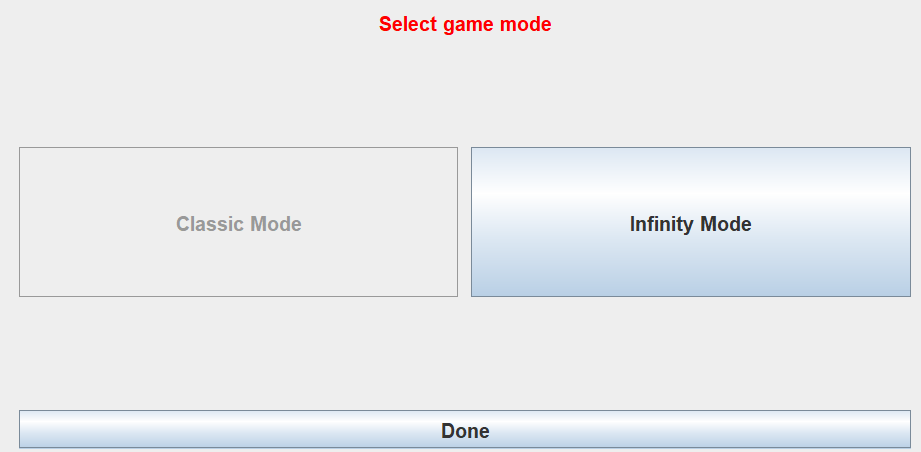
\includegraphics[width=1.3\textwidth]{img/screengame/sel_game_mod.png}}	
    \caption{schermata di selezione modalità di gioco}
	\label{img:gamescreen3}
\end{figure}
\subsection{IInterfaccia Grafica e Schermate Principali}
L’interfaccia grafica è suddivisa in aree funzionali:\newline
\begin{itemize}
    \item Tabellone:\newline
    Visualizza tutte le caselle, token, proprietà e miglioramenti.\newline Segna graficamente l'acquisto di una proprietà tramite dei badge del colore del proprietario. Similmente segnala anche case e hotel tramite delle lable.
    \item Pannello giocatore:\newline
    Mostra nome, identificativo numerico e saldo attuale del giocatore attivo.
    \item Pannelli centrali:\newline
    composto dai seguenti:\newline
    Azioni contestuali: mostra i pulsanti per eseguire azioni (compra proprietà, compra casa, compra hotel, paga affitto).\newline
    Dettaglio carta: visualizza la carta ingrandita della casella con info su affitti, proprietario, valore.
    \item Comandi principali:\newline
    sono incapsulati nei bottoni:\newline
    Tira dadi: tira i dadi e avvia il movimento\newline
    Gestione Proprietà: consente la gestione e vendita dei beni posseduti\newline
    Termina turno: termina il turno se tutte le azioni obbligatorie sono concluse (pagamento affitti, tiro dei dadi, eventuali effetti speciali)\newline
    "?": visualizza il regolamento
\end{itemize}
\begin{figure}[H]
    \centering
    \makebox[0.25\textwidth]{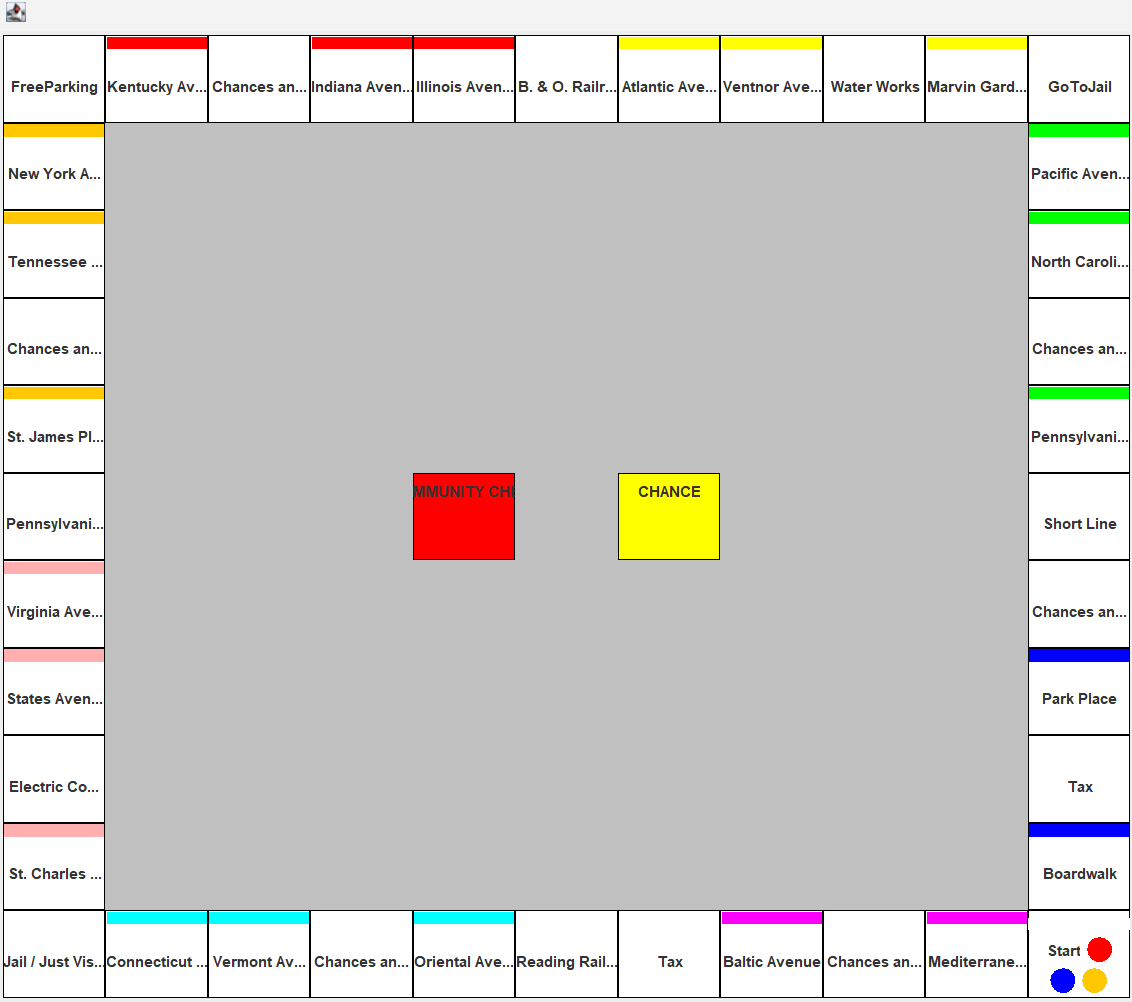
\includegraphics[width=1.3\textwidth]{img/screengame/game_board.png}}	
    \caption{il tebellone di gioco}
	\label{img:gamescreen4}
\end{figure}
\begin{figure}[H]
    \centering
    \makebox[0.5\textwidth]{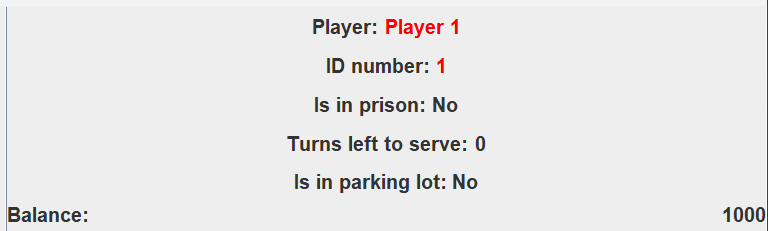
\includegraphics[width=1.3\textwidth]{img/screengame/player_info.png}}	
    \caption{pannello con le informazioni relative al player che sta giocando il turno}
	\label{img:gamescreen5}
\end{figure}
\begin{figure}[H]
    \centering
    \makebox[0.5\textwidth]{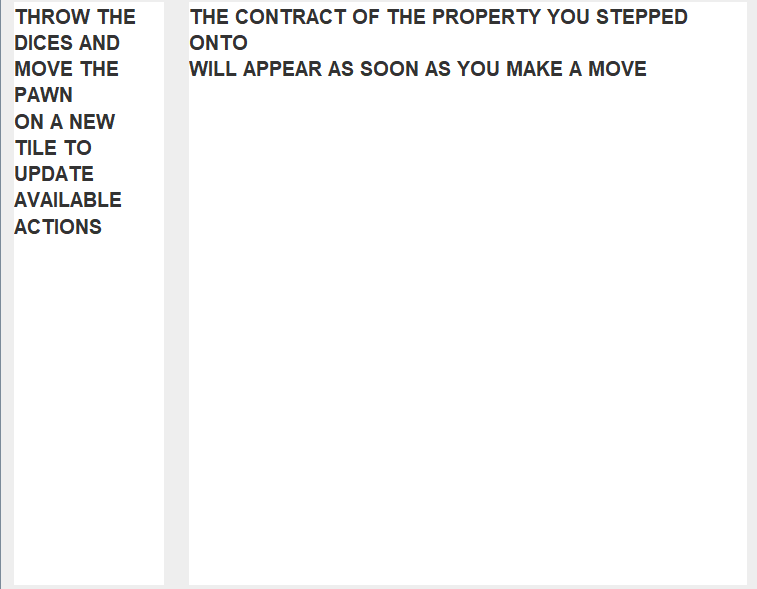
\includegraphics[width=1.3\textwidth]{img/screengame/property_info.png}}	
    \caption{pannello con le informazioni relative alla proprietà su cui si trova il player e le possibili azioni}
	\label{img:gamescreen6}
\end{figure}
\begin{figure}[H]
    \centering
    \makebox[1\textwidth]{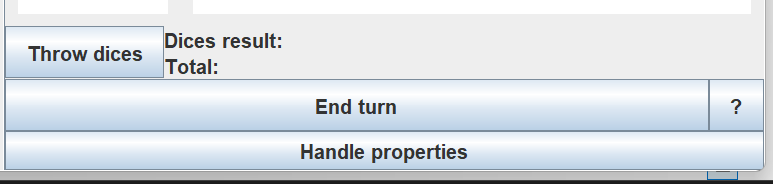
\includegraphics[width=1.3\textwidth]{img/screengame/action_buttons.png}}	
    \caption{pannello con le informazioni relative al player che sta giocando il turno}
	\label{img:gamescreen7}
\end{figure}
\subsection{Svolgimento del turno}
Ogni turno si compone di:
\begin{enumerate}
    \item Fase pre-tiro (facoltativa): vendita di beni tramite "Gestione Proprietà".
    \item Tiro dei dadi: clic su "Tira dadi", movimento sul tabellone.
    \item Interazione con la casella: acquisto, pagamento affitto, carte evento, tasse, acquisti di case/hotel se applicabili.
    \item Consultazione dettagli: tramite pannello carta ingrandita.
    \item Fine turno: clic su "Termina turno"; in Classic Mode è obbligatorio avere saldo positivo per non perdere.
\end{enumerate}
\subsection{Proprietà e Miglioramenti}
Le azioni eseguibili sulle proprietà sono:
\begin{itemize}
    \item Acquisto: Si possono comprare proprietà solo se non possedute da altri giocatori.
    \item Affitti: Vengono pagati tramite la banca,\newline il loro valore raddoppia nel caso in cui il proprietario dovesse aver comprato tutte le proprietà di uno stesso gruppo e aumenta ulteriormente se si dovessero costruire case o alberghi.
    \item Costruzione di case e hotel: Per poter costruire è necessario possedere tutte le proprietà di uno stesso gruppo/colore ed essere sulla proprietà su cui si vuole erigere la casa (o l'hotel).\newline Per costruire un hotel è necessario aver acquistato 4 case (il massimo di case sulla proprietà).
    \item Vendite: è possibile vendere le proprietà accquistate in precedenza e le costruzioni in una finestra dedicata, il valore di vendità diminuisce rispetto a quello d'acquisto.\newline
    Le Case e gli Hotel restituiscono il 50\% del loro valore di acquisto.\newline
    Le Proprietà, vendibili solo se prive di case/hotel, restituiscono il 50\% del loro valore di acquisto.\newline
    Le Stazioni restituiscono il 75\% del loro valore di acquisto.
\end{itemize}
\begin{figure}[H]
    \centering
    \makebox[0.5\textwidth]{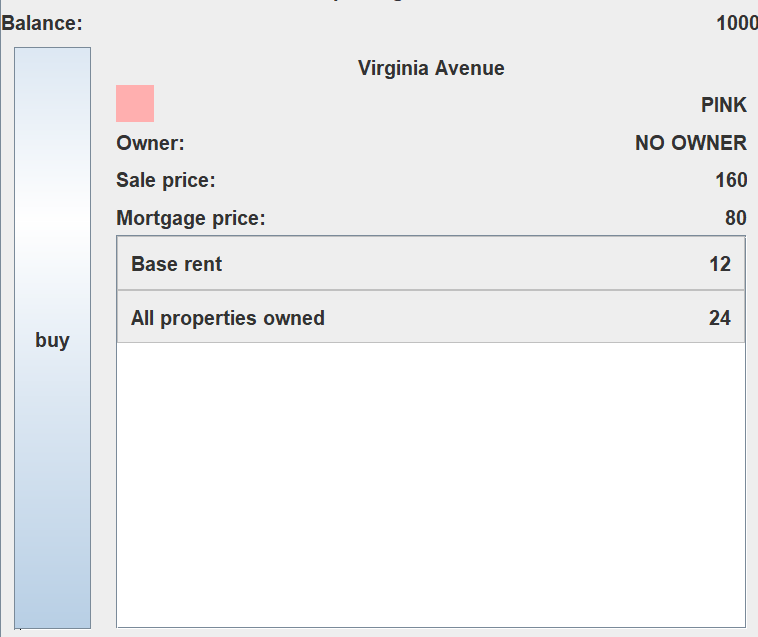
\includegraphics[width=1\textwidth]{img/screengame/buy_property.png}}	
    \caption{situazione in cui si può comprare un aproprietà}
	\label{img:gamescreen8}
\end{figure}
\begin{figure}[H]
    \centering
    \makebox[0.5\textwidth]{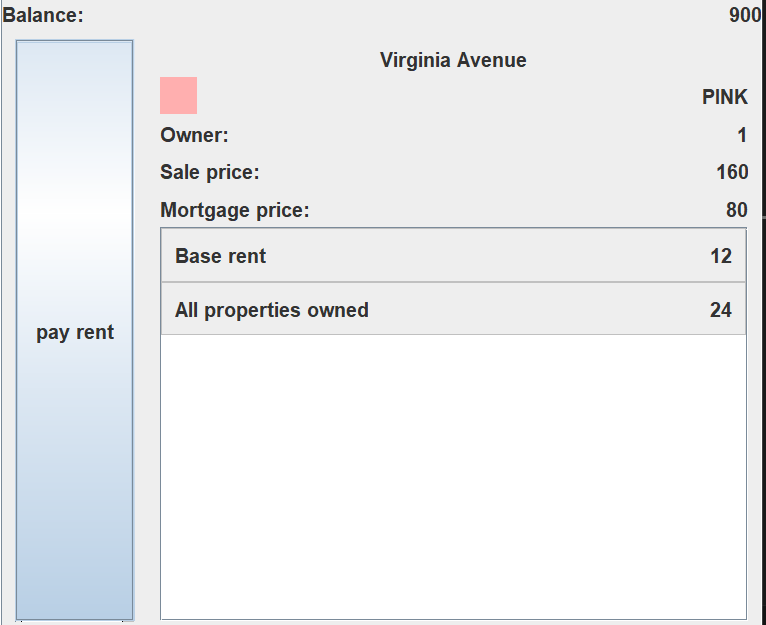
\includegraphics[width=1\textwidth]{img/screengame/pay_rent.png}}	
    \caption{situazione in cui si deve pagare l'affitto della proprietà}
	\label{img:gamescreen9}
\end{figure}
\begin{figure}[H]
    \centering
    \makebox[0.5\textwidth]{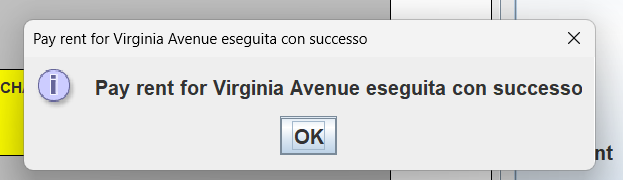
\includegraphics[width=1\textwidth]{img/screengame/rent_payment_confirm.png}}	
    \caption{esempio di conferma avvenuto pagamento}
	\label{img:gamescreen10}
\end{figure}
\begin{figure}[H]
    \centering
    \makebox[0.1\textwidth]{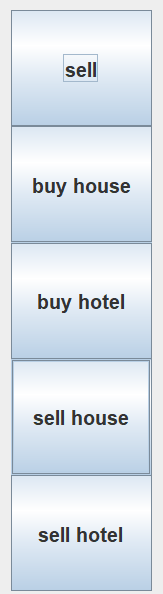
\includegraphics[width=0.15\textwidth]{img/screengame/house_hotels.png}}	
    \caption{bottoni disponibili sulle proprietà possedute una volta che si hanno tutte quelle del gruppo}
	\label{img:gamescreen11}
\end{figure}
\begin{figure}[H]
    \centering
    \makebox[0.5\textwidth]{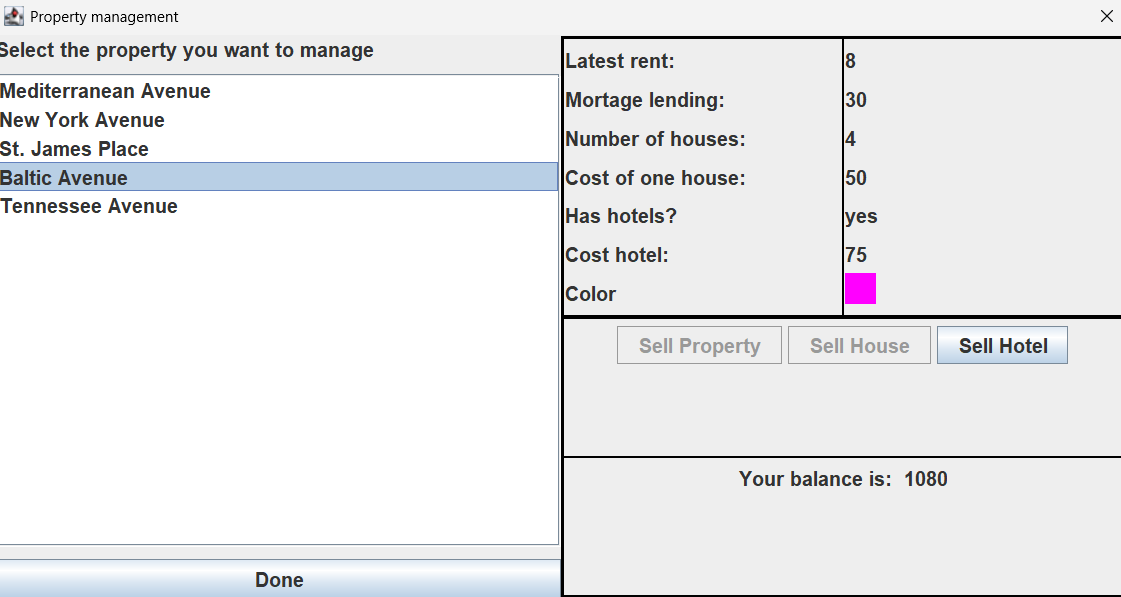
\includegraphics[width=1.3\textwidth]{img/screengame/manage_property.png}}	
    \caption{finestra per la vendita delle proprieta, delle case e degli hote}
	\label{img:gamescreen12}
\end{figure}
\subsection{Caselle Speciali}
\begin{itemize}
    \item Prigione: ci sono 2 modi di capitare su questa casella, tramite tiro del dado, non succede nulla, o tramite la casella "Go to Jail", in quel caso si rimane bloccati per 3 turni oppure,\newline se si ottiene un numero doppio ai dadi, si può evadere ignorando il numero di turni.\newline Anche essendo bloccati rimane possibile gestire le proprietà tramite l'apposito menù all'interno del proprio turno.
    \item Tasse: Le caselle Tassa impongono un pagamento imprerogabile alla banca.
    \item Imprevisti/Probabilità: Le caselle Impreviti/Probabilità fanno pescare da un deck di 20 carte, tutte con effetti che possono variare il corso del turno.\newline Una volta attivato l'effetto la carta viene reinserita nel mazzo. 
    \item Free Parking: non ha nessuna ripercussione a livello economico ma fa restare bloccato per 1 turno il player che ci capita.
    \item Società: sono dei sottotipi delle proprietà normali ma hanno l'affitto che cambia in base al tiro del dado.
    \item Stazioni: sono dei sottotipi delle proprietà normali ma il loro affitto raddoppia ogni volta che compri una proprieta di tipo stazione.
\end{itemize}
\begin{figure}[H]
    \centering
    \makebox[0.5\textwidth]{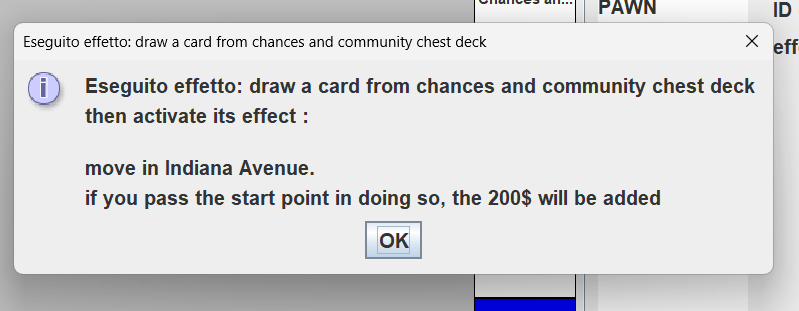
\includegraphics[width=1.3\textwidth]{img/screengame/effect_Activated.png}}	
    \caption{esempio di attivazione dell'effetto di una carta imprevito-probabilità}
	\label{img:gamescreen13}
\end{figure}
\begin{figure}[H]
    \centering
    \makebox[0.5\textwidth]{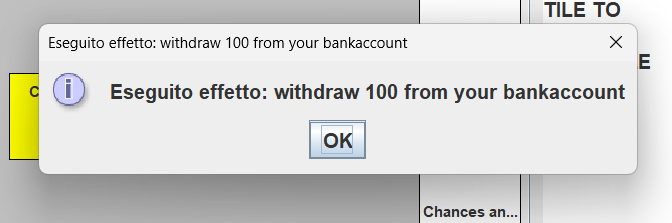
\includegraphics[width=1.3\textwidth]{img/screengame/withdraw_effect.png}}	
    \caption{esempio di attivazione dell'effetto di una casella Tassa}
	\label{img:gamescreen14}
\end{figure}
\subsection{Fine del gioco e condizioni di vittoria}
\begin{itemize}
    \item Classic Mode: Per vincere facendo finire il gioco si deve far in modo di essere l'unico giocatore sul tabellone ovvero l'unico con il saldo in positivo in quanto\newline se si dovesse terminare il turno con saldo negativo si verrebbe eliminati.
    \item Infinity Mode: Per vincere facendo finire il gioco si deve fare in modo di essere il giocatore con il patrimonio monetrio più alto in quanto in questa modalità non ci sono eliminazioni di alcun tipo.
\end{itemize}
I giocatori possono sempre terminare la partita utilizzando la "X" della finestra di gioco, in quel caso vince il giocatore con il saldo più alto.
\subsection{Riepilogo Comandi e Struttura Tecnica}
Pulsanti principali: Tira dadi, Gestione Proprietà, Termina turno, "?".
Azioni contestuali (casella attuale): Buy Property, Buy House, Buy Hotel, Pay Rent, Sell House, Sell Hotel, Sell Property.\newline 
Regolamento: Sempre accessibile tramite "?" in qualsiasi momento e caricato dal percorso indicato nel campo RULESFILE.\newline 
Parametri personalizzabili dal file di configurazione: numero giocatori, dadi, saldo iniziale, font, percorsi ai file, colori dei token dei giocatori
\chapter{Esercitazioni di laboratorio}
\section{davide.rossi47@studio.unibo.it}
\begin{itemize}
    \item Laboratorio 07: \url{https://virtuale.unibo.it/mod/forum/discuss.php?d=177162#p246183}
    \item Laboratorio 08: \url{https://virtuale.unibo.it/mod/forum/discuss.php?d=178723#p247214}
    \item Laboratorio 09: \url{https://virtuale.unibo.it/mod/forum/discuss.php?d=179154#p248357}
    \item Laboratorio 10: \url{https://virtuale.unibo.it/mod/forum/discuss.php?d=180101#p249538}
\end{itemize}
\section{alessio.minniti@studio.unibo.it}
\begin{itemize}
    \item Laboratorio 08: \url{https://virtuale.unibo.it/mod/forum/discuss.php?d=178723#p247295}
    \item Laboratorio 09: \url{https://virtuale.unibo.it/mod/forum/discuss.php?d=179154#p248022}
    \item Laboratorio 10: \url{https://virtuale.unibo.it/mod/forum/discuss.php?d=180101#p249462}
    \item Laboratorio 11: \url{https://virtuale.unibo.it/mod/forum/discuss.php?d=181206#p250861}
\end{itemize}